\documentclass{beamer}
\usetheme{Antibes}
\setbeamertemplate{navigation symbols}{} 
\usepackage{amsmath}
\usepackage[T1]{fontenc}
\usepackage{lmodern}
% \usepackage{showframe}

\usepackage{graphicx}
\graphicspath{{.}{images/}}

\setbeamertemplate{caption}{\raggedright\insertcaption\par}

\title[Optimized Software for Theoretical Nonlinear Optical Calculations
\hspace{5.5cm}\insertframenumber/\inserttotalframenumber]
{Optimized Software for Theoretical Nonlinear Optical Calculations}
\author{\texorpdfstring{Sean M. Anderson\vspace{-0.7em}}{Sean M. Anderson}}
\institute{Centro de Investigaciones en \'Optica, A.C\vspace{-1em}}
\date{\small\today\vspace{-1.2em}}
\titlegraphic{
\begin{figure}
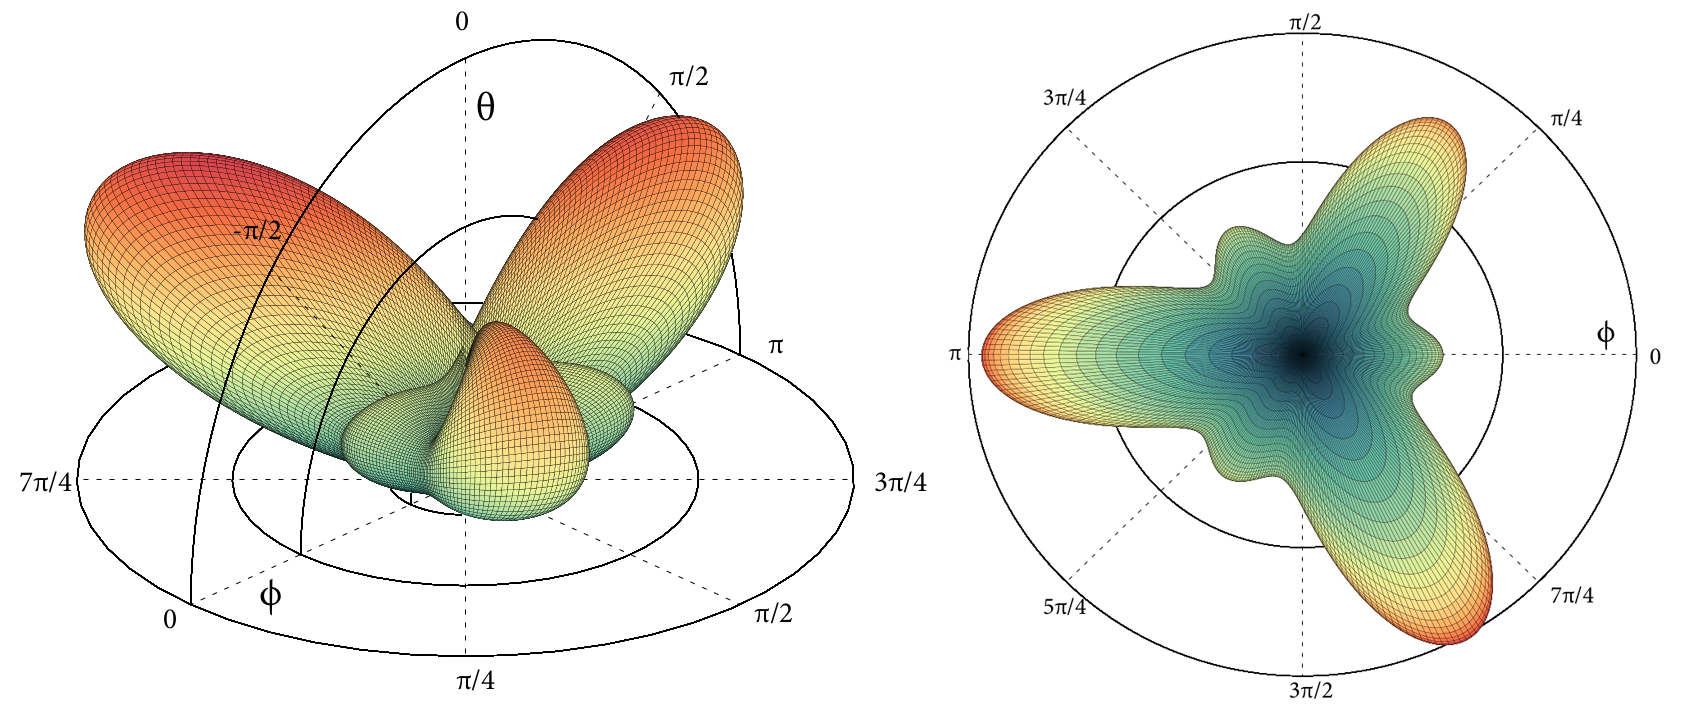
\includegraphics[width=0.8\textwidth]{3D-cover}
\end{figure}}


\begin{document}

\begin{frame}
\maketitle
\end{frame}

%%%%%%%%%%%%%%%%%%%%%%%%%%%%%%%%%%%%%%%%%%%%%%%%%%%%%%%%%%%%%%%%%%%%%%%%%%%%%%%%
%%%%%%%%%%%%%%%%%%%%%%%%%%%%%%%%%%%%%%%%%%%%%%%%%%%%%%%%%%%%%%%%%%%%%%%%%%%%%%%%

\section{Introduction}

\begin{frame}
\frametitle{Second Harmonic Generation (SHG)}
\begin{block}{Characteristics\footnote{Image: Jon Chui}}
\begin{itemize}
\item Two photons of the same frequency combine
\item Create one photon of double the frequency
\end{itemize}
\end{block}
\begin{figure}
\centering
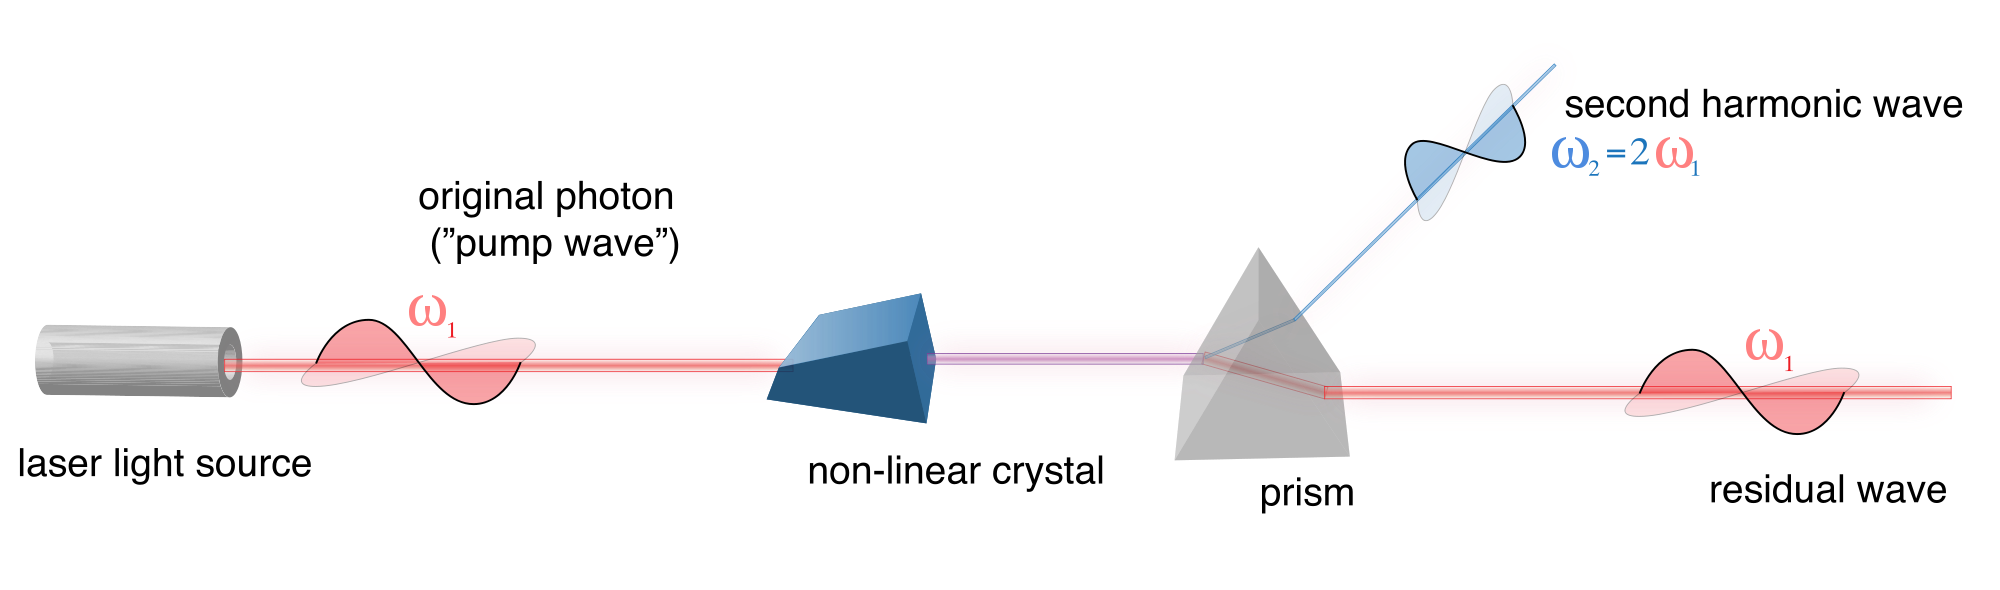
\includegraphics[width=0.9\textwidth]{diag-shg}
\end{figure}
\end{frame}

\begin{frame}
% \frametitle{A two column slide}
\begin{columns}
\column{0.5\textwidth}
\begin{figure}
\centering
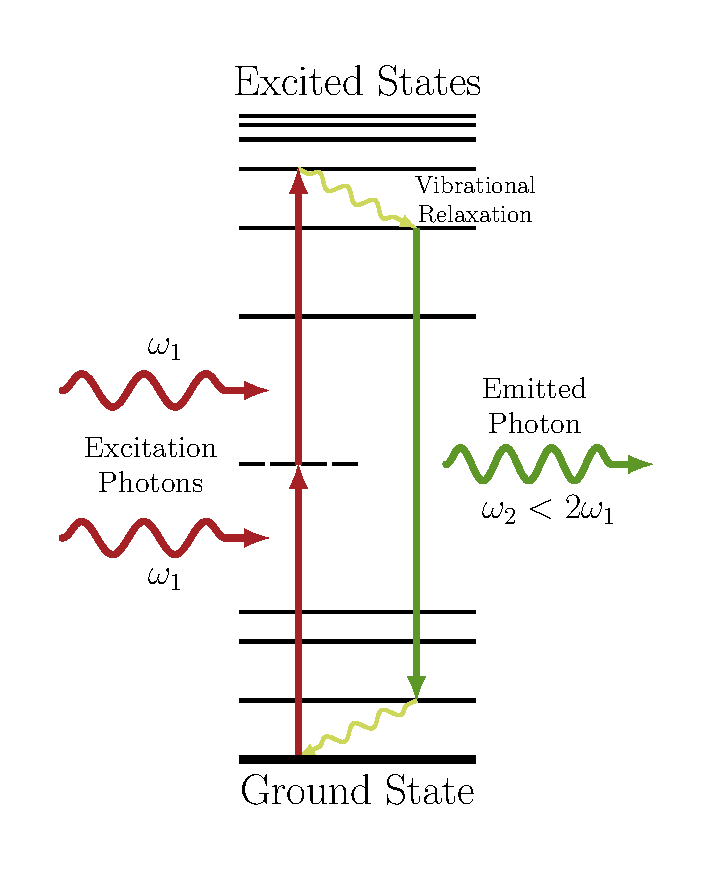
\includegraphics[width=\textwidth]{diag-levelsflourescence}
\end{figure}
\column{0.5\textwidth}
\begin{figure}
\centering
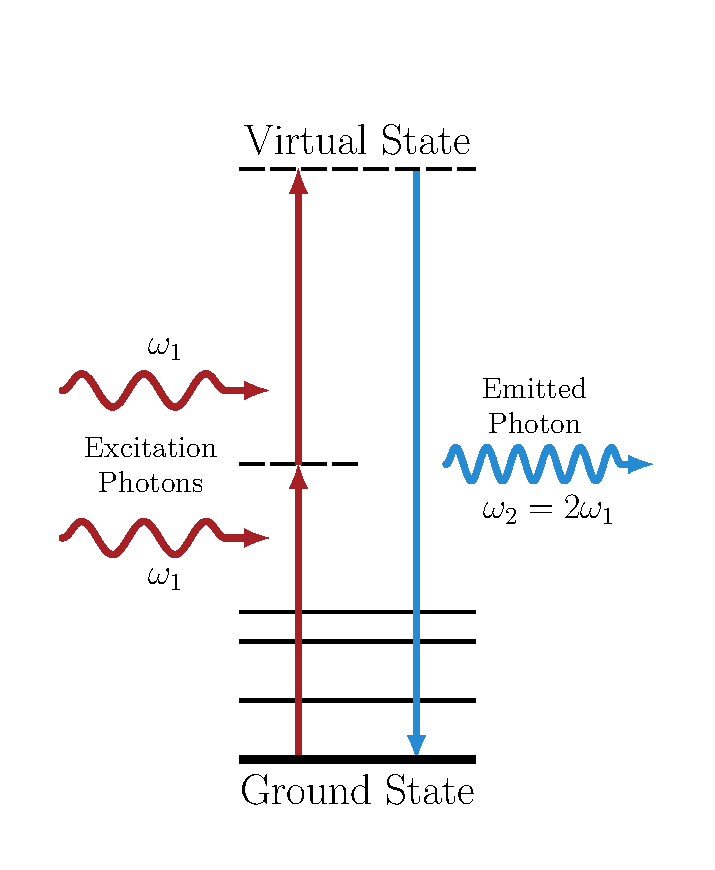
\includegraphics[width=\textwidth]{diag-levelsshg}
\end{figure}
\end{columns}
\end{frame}

\begin{frame}
\frametitle{Second-order Nonlinear Effects}
Early work\footnote{J.A. Armstrong et al. \emph{Physical Review}, 127(6):1918--1939, Sep 1962.} \footnote{N. Bloembergen et al. \emph{Physical Review}, 128(2):606--622, Oct 1962.} demonstrated that second-order processes
\begin{itemize}
\item Are dipole forbidden in the bulk of centrosymmetric materials
\item Are related to $\chi^{(2)}$, the nonlinear susceptibility
\item Have bigger dipolar (surface) than quadrupolar contributions
\end{itemize}\vfill
\begin{center}
Second-order processes are well studied for flat surfaces, but what about round materials like nanospheres?
\end{center}
\end{frame}

\begin{frame}
\frametitle{Summary}
\begin{block}{Nonlinear response depends on}
\begin{itemize}
\item Nonlocal excitation of the electric dipole moment 
\item Local excitation of the electric quadrupole moment
\item The strength of the incident beam and
\item The form (plane wave, Gaussian beam, polarization, etc.)
\item The quadrupolar $\left(\mathbf{E}\cdot\nabla\right)\mathbf{E}$ term
\end{itemize}
\end{block}
What's the best way to enhance this signal?
\end{frame}

\begin{frame}
\frametitle{Centrosymmetric Materials}
A centrosymmetric material is a material that displays inversion symmetry, such
that $p(x,y,z) \rightarrow p(-x,-y,-z)$.
\begin{columns}
\column{0.5\textwidth}
\begin{figure}
\centering
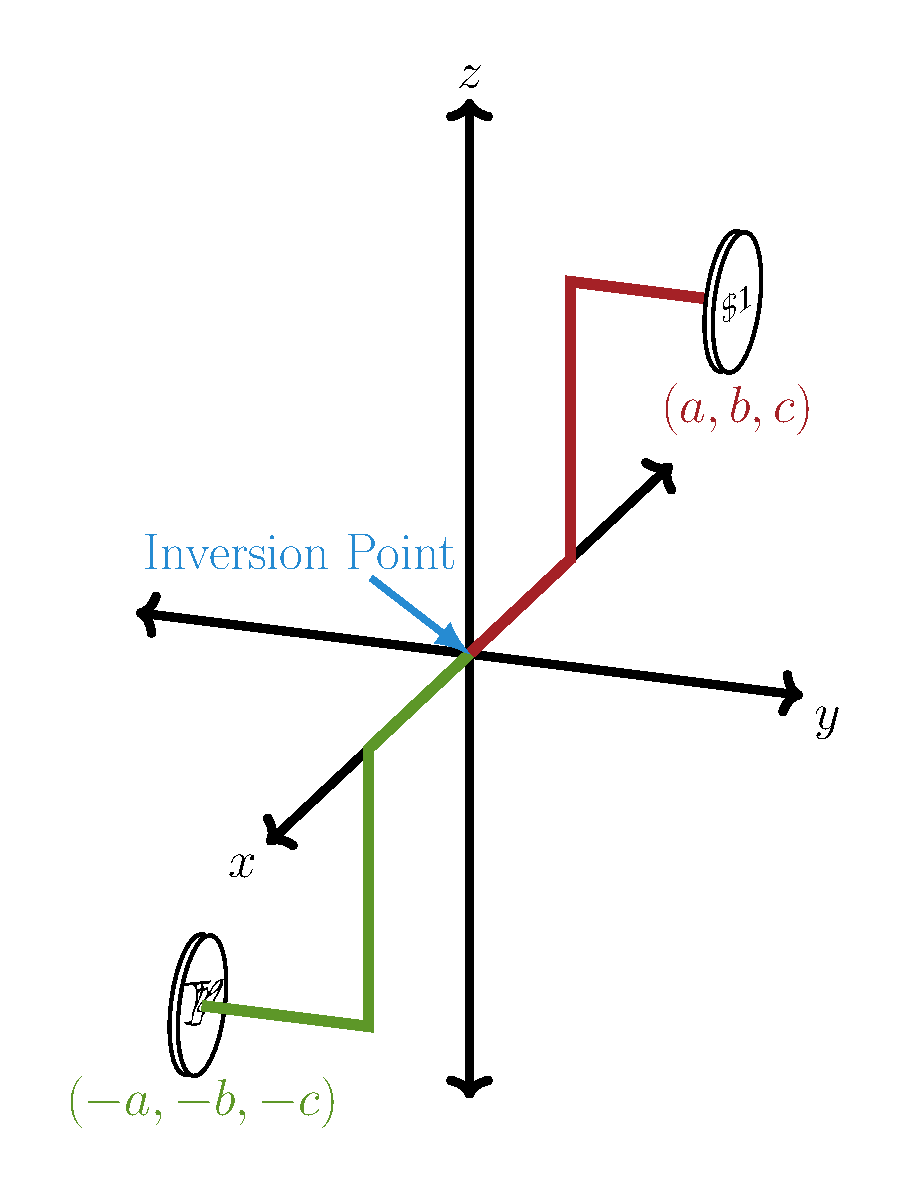
\includegraphics[width=0.7\textwidth]{diag-centrosymmetry}
\end{figure}
\column{0.5\textwidth}
\begin{itemize}
\item Many nonlinear materials are centrosymmetric
\item Nanospheres are definitely centrosymmetric
\item The material in these nanoparticles is centrosymmetric
\end{itemize}
\end{columns}
\end{frame}

\begin{frame}
\frametitle{Test Cases}
\begin{columns}
\column{0.5\textwidth}
\begin{figure}
\centering
\includegraphics[height=0.7\textheight]{struc-Si2x1-front}
\caption{Si(001)(2$\times$1)}
\end{figure}
\column{0.5\textwidth}
\begin{figure}
\centering
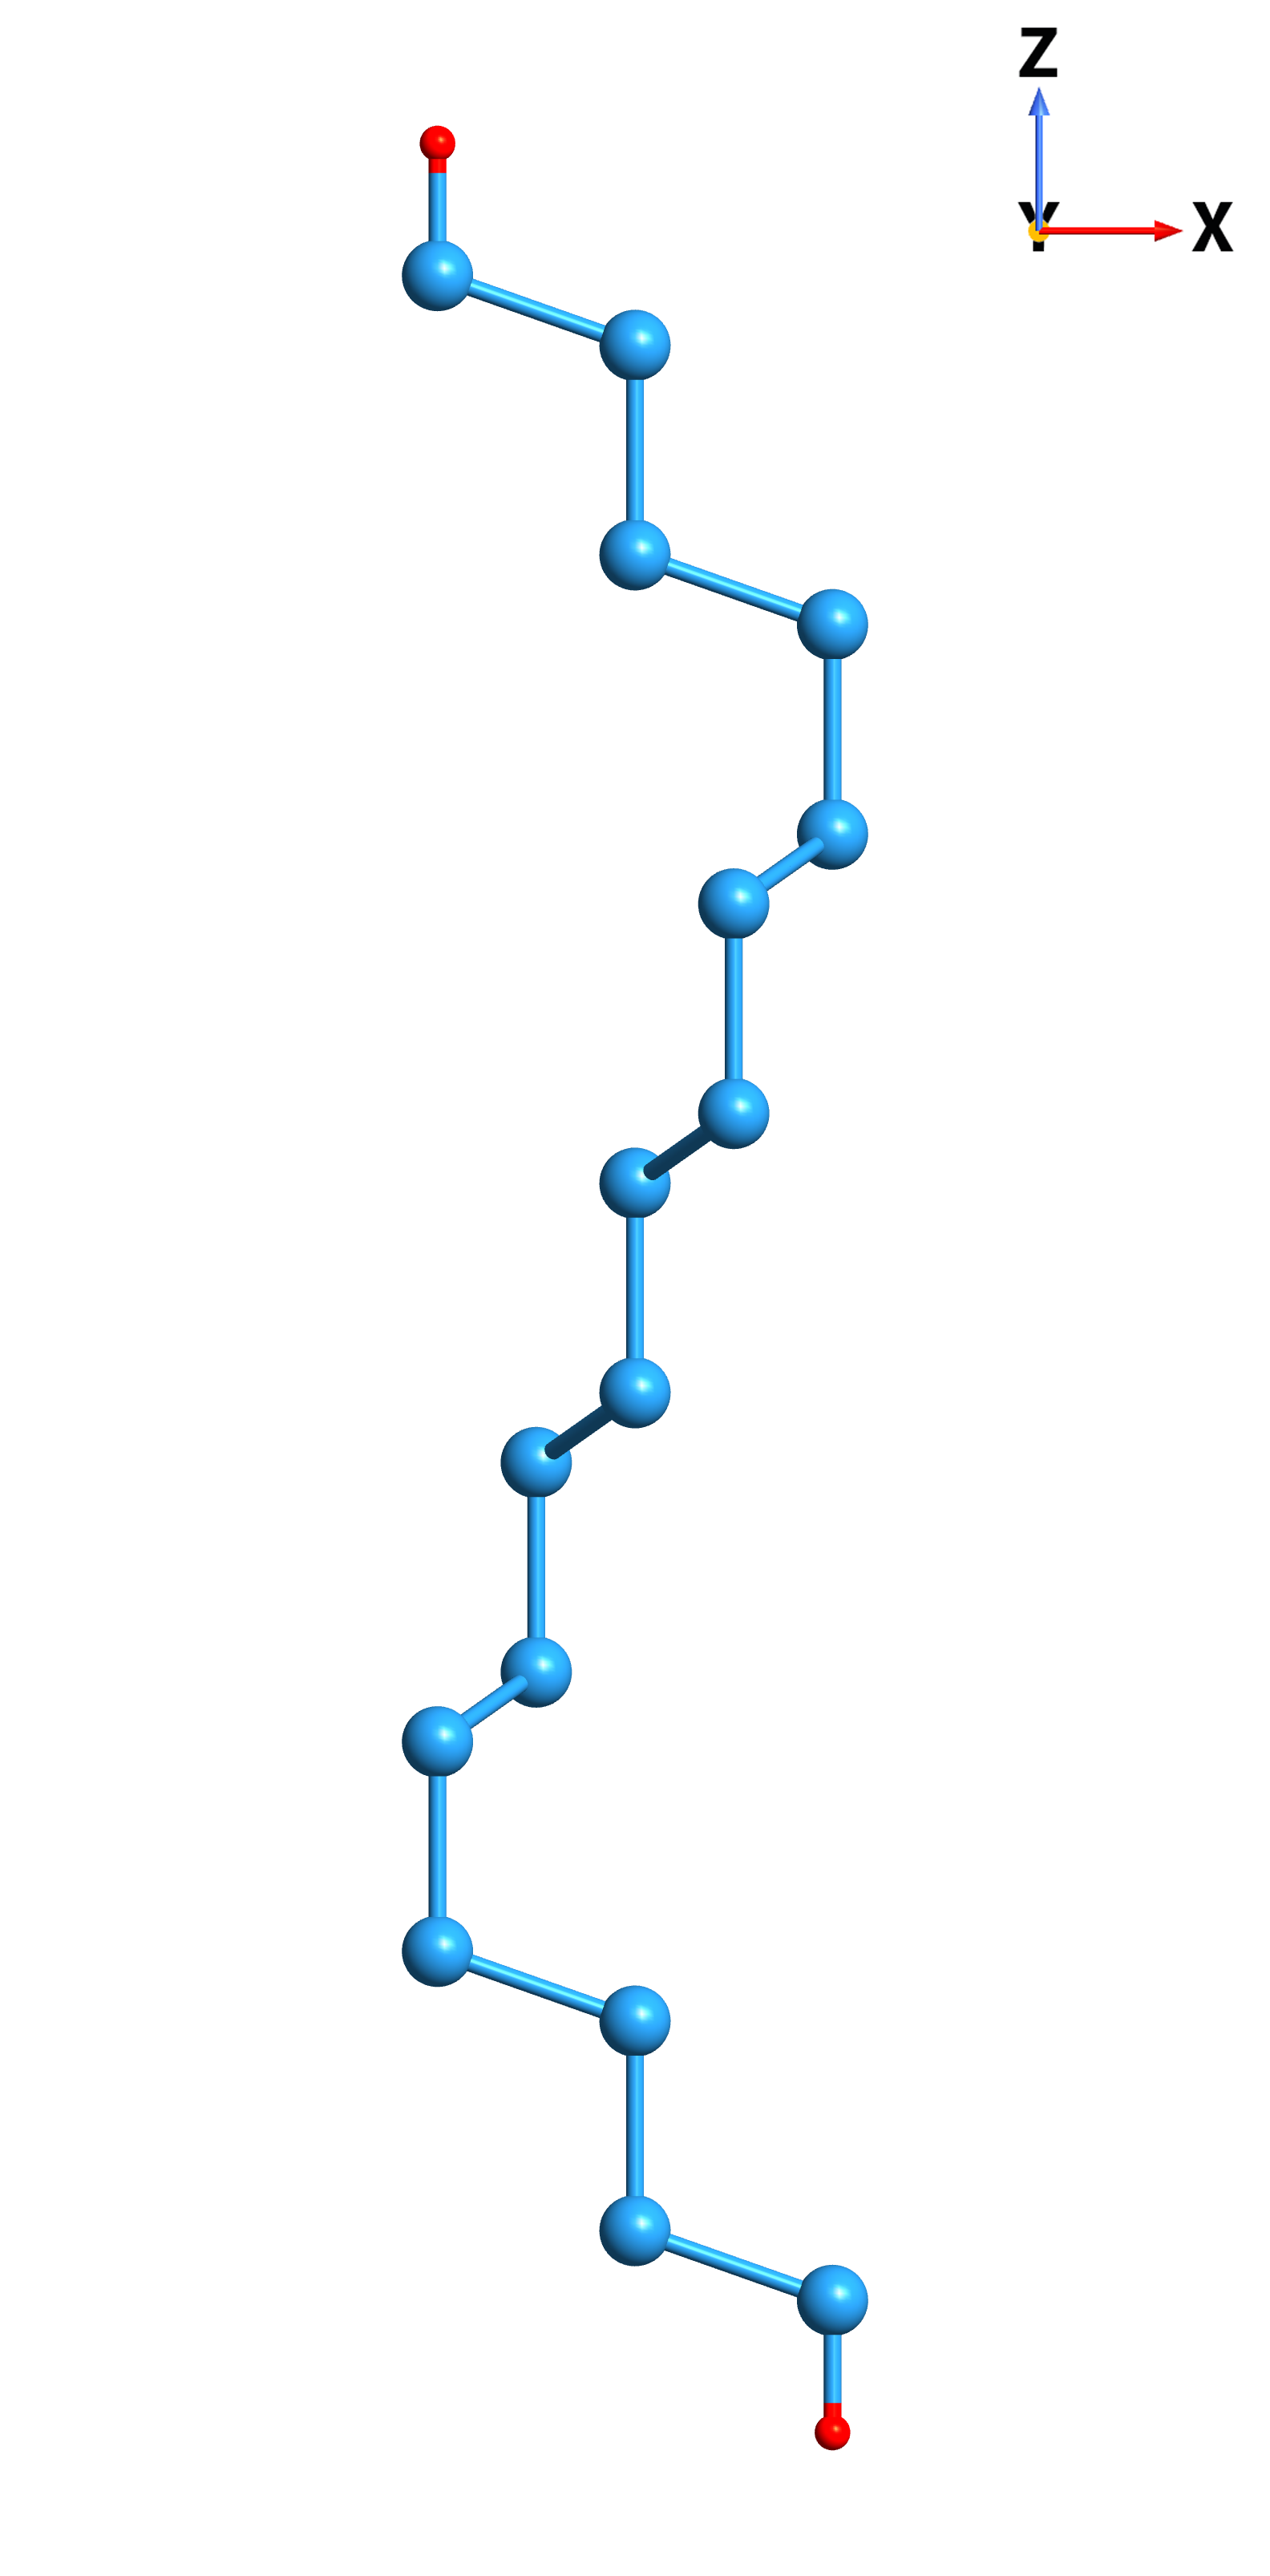
\includegraphics[height=0.7\textheight]{struc-Si1x1-front}
\caption{Si(111)(1$\times$1):H}
\end{figure}
\end{columns}
\end{frame}


%%%%%%%%%%%%%%%%%%%%%%%%%%%%%%%%%%%%%%%%%%%%%%%%%%%%%%%%%%%%%%%%%%%%%%%%%%%%%%%%
%%%%%%%%%%%%%%%%%%%%%%%%%%%%%%%%%%%%%%%%%%%%%%%%%%%%%%%%%%%%%%%%%%%%%%%%%%%%%%%%

\section{Chi2}

\begin{frame}
% \frametitle{A two column slide}
\begin{figure}
\centering
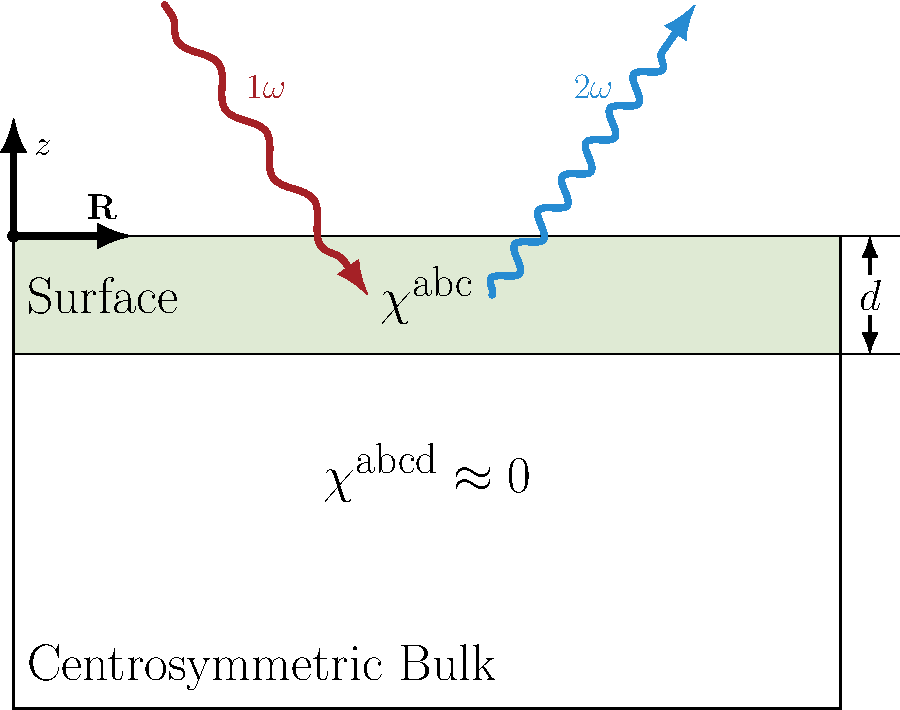
\includegraphics[width=\textwidth]{diag-system}
\end{figure}
\end{frame}

\begin{frame}
% \frametitle{A two column slide}
\begin{figure}
\centering
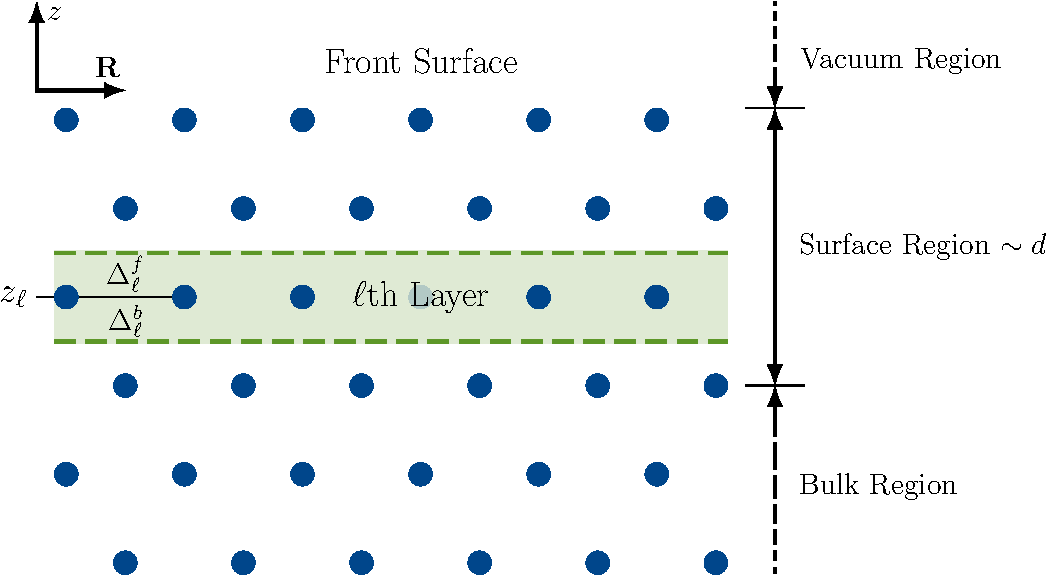
\includegraphics[width=\textwidth]{diag-slab}
\end{figure}
\end{frame}

\begin{frame}
% \frametitle{A two column slide}
\begin{figure}
\centering
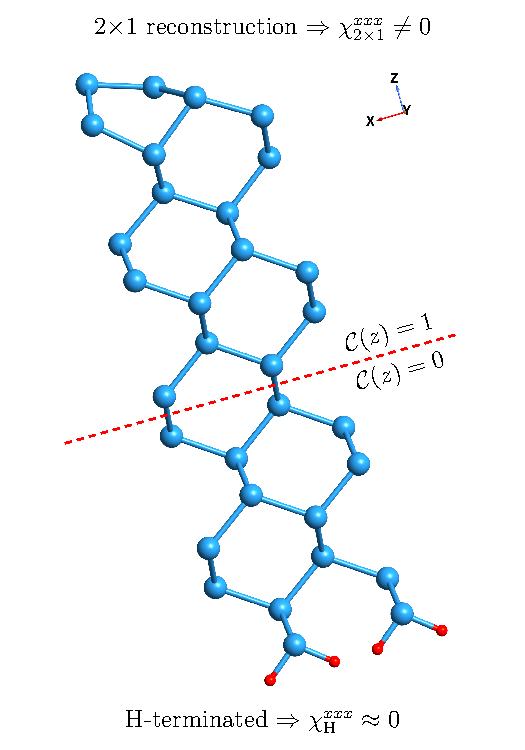
\includegraphics[height=0.9\textheight]{struc-Si2x1-rot}
\end{figure}
\end{frame}

\begin{frame}
% \frametitle{A two column slide}
\begin{figure}
\centering
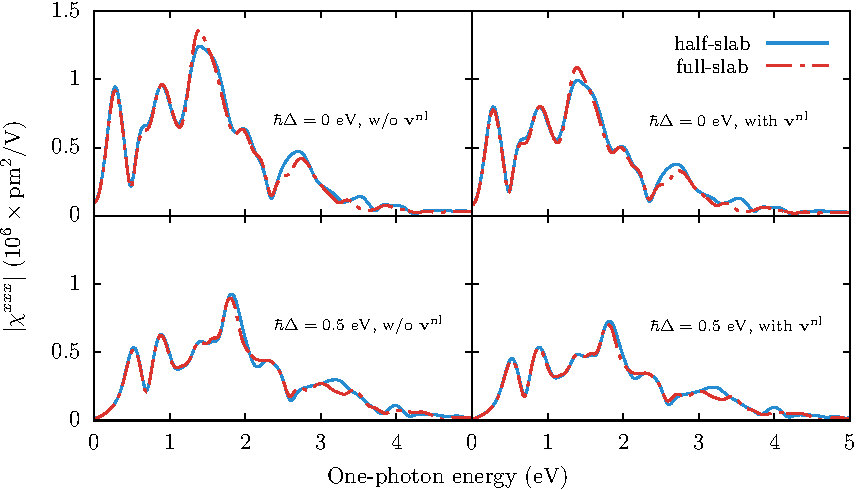
\includegraphics[width=\textwidth]{fig-Si2x1-hsvsfs}
\end{figure}
\end{frame}

\begin{frame}
% \frametitle{A two column slide}
\begin{figure}
\centering
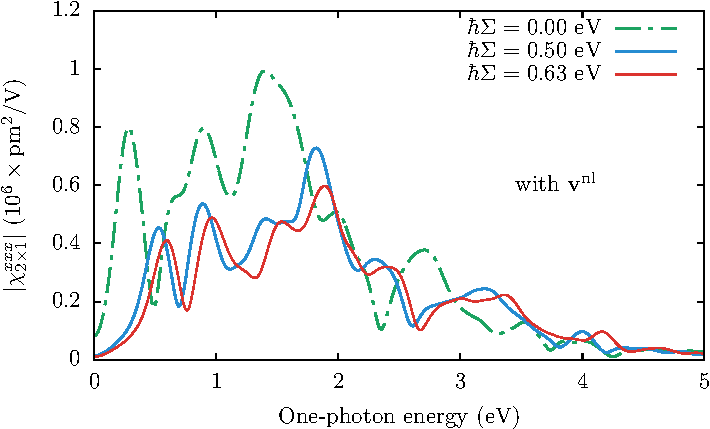
\includegraphics[width=\textwidth]{fig-Si2x1-scissors}
\end{figure}
\end{frame}

\begin{frame}
% \frametitle{A two column slide}
\begin{figure}
\centering
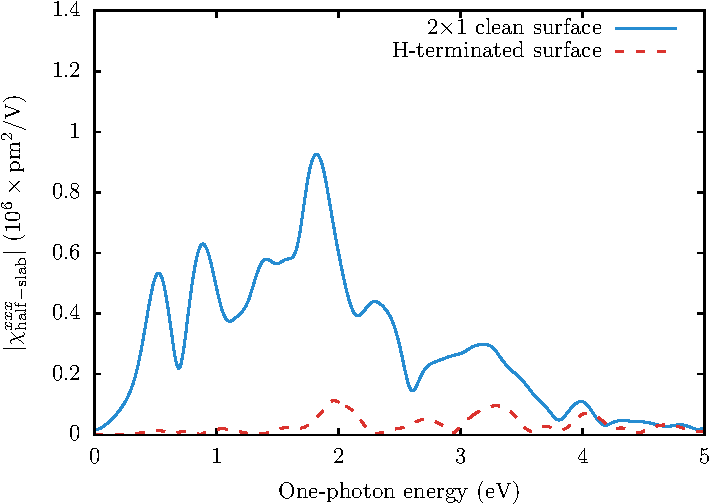
\includegraphics[width=\textwidth]{fig-Si2x1-topvbottom}
\end{figure}
\end{frame}

\begin{frame}
% \frametitle{A two column slide}
\begin{figure}
\centering
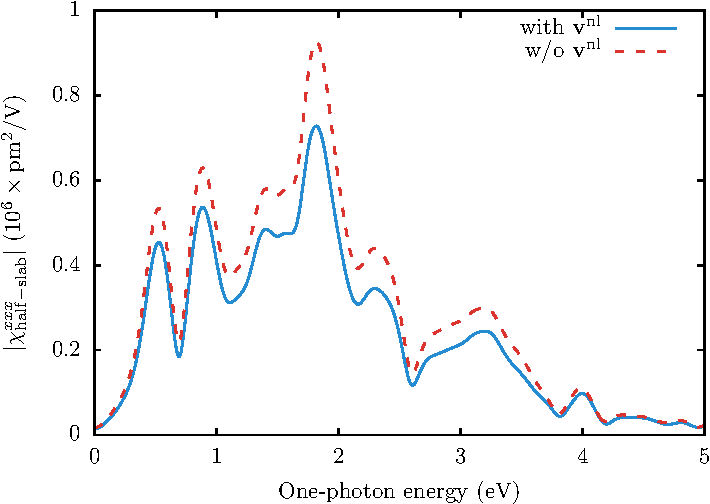
\includegraphics[width=\textwidth]{fig-Si2x1-vnl}
\end{figure}
\end{frame}

\begin{frame}
% \frametitle{A two column slide}
\begin{figure}
\centering
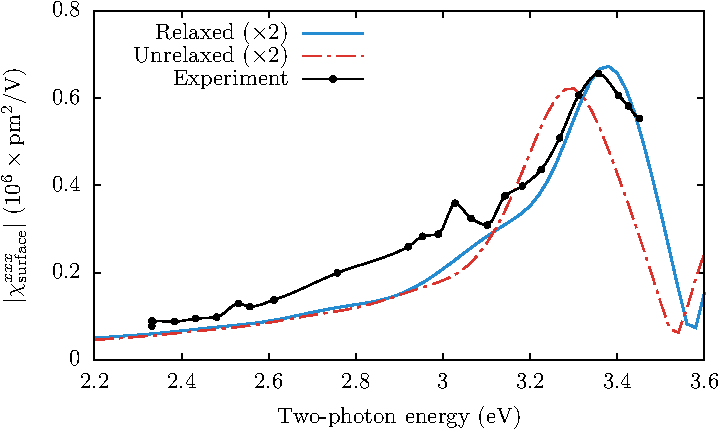
\includegraphics[width=\textwidth]{fig-Si1x1-Hofer_Xxxx}
\end{figure}
\end{frame}


%%%%%%%%%%%%%%%%%%%%%%%%%%%%%%%%%%%%%%%%%%%%%%%%%%%%%%%%%%%%%%%%%%%%%%%%%%%%%%%%
%%%%%%%%%%%%%%%%%%%%%%%%%%%%%%%%%%%%%%%%%%%%%%%%%%%%%%%%%%%%%%%%%%%%%%%%%%%%%%%%

\section{SSHG Yield}

\begin{frame}
% \frametitle{A two column slide}
\begin{figure}
\centering
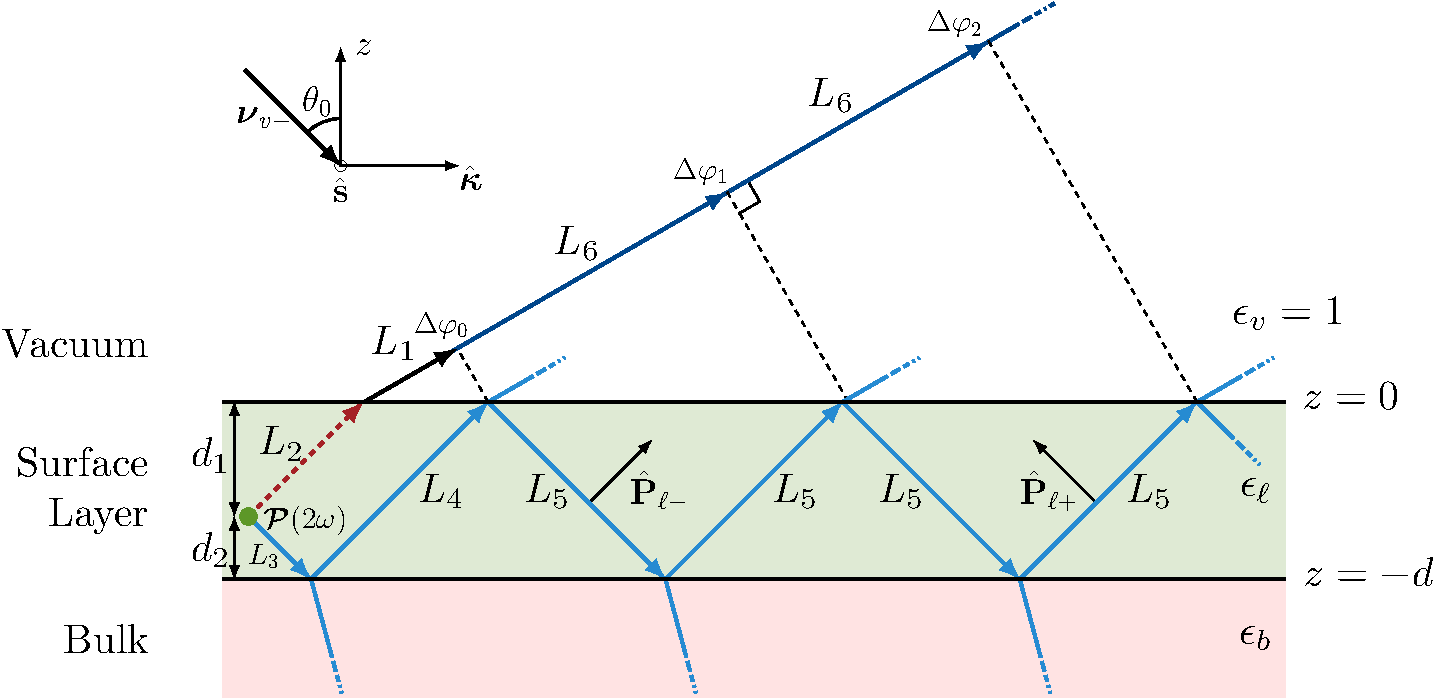
\includegraphics[width=\textwidth]{diag-3layer_MR_2w}
\end{figure}
\end{frame}

\begin{frame}
% \frametitle{Test Cases}
\begin{columns}
\column{0.5\textwidth}
\begin{figure}
\centering
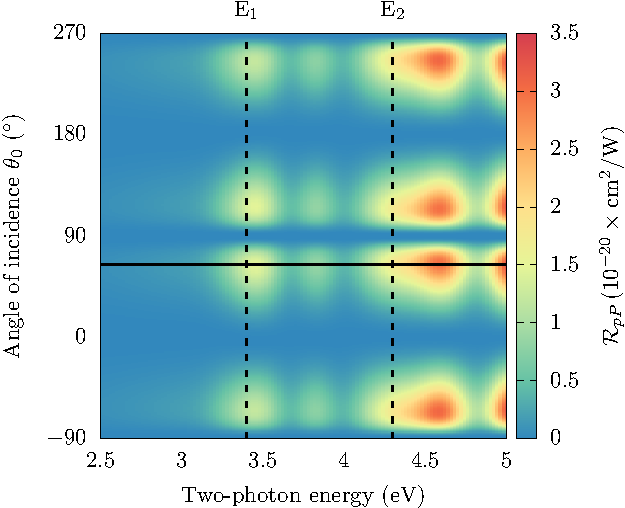
\includegraphics[width=\textwidth]{3D-Si1x1-RpP}
\end{figure}
\column{0.5\textwidth}
\begin{figure}
\centering
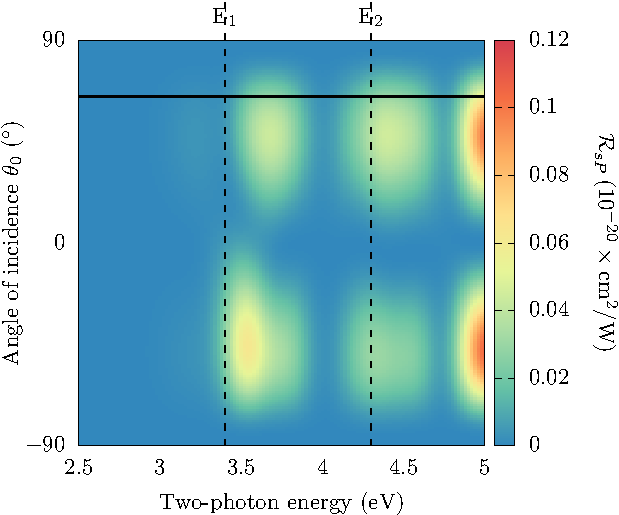
\includegraphics[width=\textwidth]{3D-Si1x1-RsP}
\end{figure}
\end{columns}
\end{frame}

\begin{frame}
% \frametitle{A two column slide}
\begin{figure}
\centering
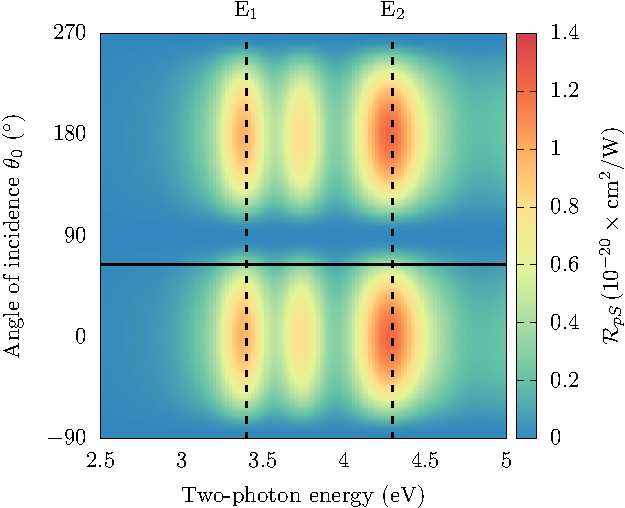
\includegraphics[width=0.5\textwidth]{3D-Si1x1-RpS}
\end{figure}
\end{frame}

\begin{frame}
% \frametitle{A two column slide}
\begin{figure}
\centering
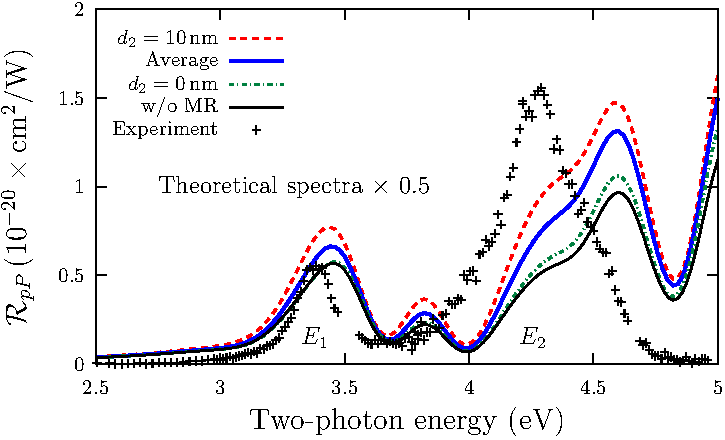
\includegraphics[width=\textwidth]{fig-Si1x1-MRdepth}
\end{figure}
\end{frame}

\begin{frame}
% \frametitle{A two column slide}
\begin{columns}
\column{0.5\textwidth}
\begin{figure}
\centering
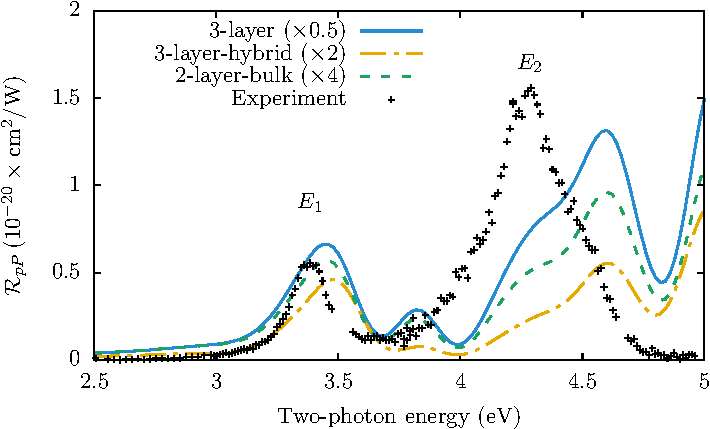
\includegraphics[width=\textwidth]{fig-Si1x1-Mejia_RpP}
\end{figure}
\column{0.5\textwidth}
\begin{figure}
\centering
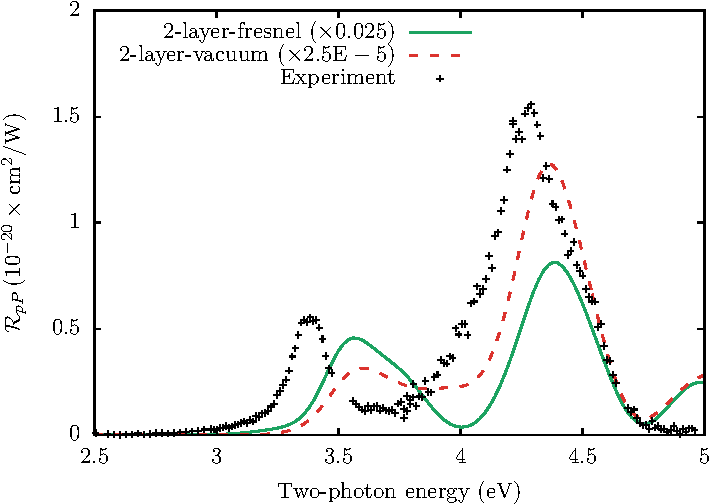
\includegraphics[width=\textwidth]{fig-Si1x1-Mejia_RpP_models}
\end{figure}
\end{columns}
\end{frame}

\begin{frame}
% \frametitle{A two column slide}
\begin{figure}
\centering
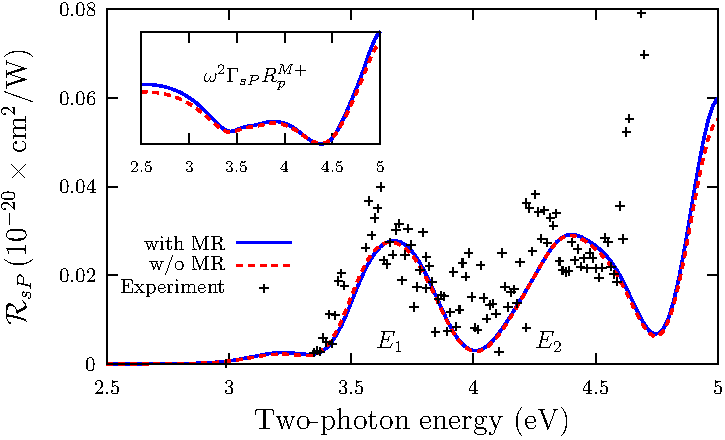
\includegraphics[width=\textwidth]{fig-Si1x1-Mejia_RsP}
\end{figure}
\end{frame}

\begin{frame}
% \frametitle{A two column slide}
\begin{figure}
\centering
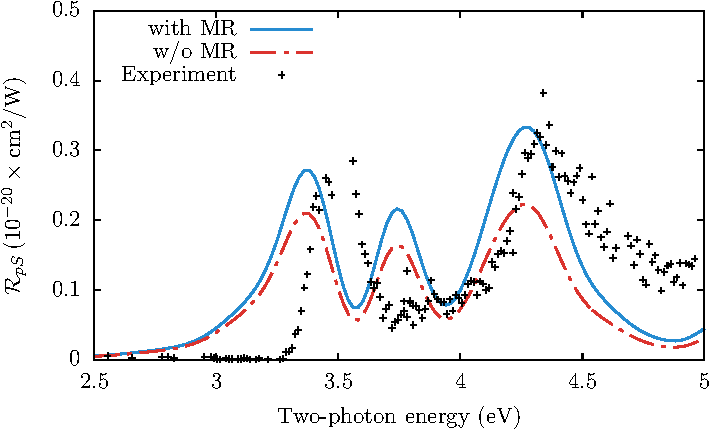
\includegraphics[width=\textwidth]{fig-Si1x1-Mejia_RpS}
\end{figure}
\end{frame}


%%%%%%%%%%%%%%%%%%%%%%%%%%%%%%%%%%%%%%%%%%%%%%%%%%%%%%%%%%%%%%%%%%%%%%%%%%%%%%%%
%%%%%%%%%%%%%%%%%%%%%%%%%%%%%%%%%%%%%%%%%%%%%%%%%%%%%%%%%%%%%%%%%%%%%%%%%%%%%%%%

\section{Conclusions}

\subsection{Chi2}
\begin{frame}
\frametitle{Title}
\begin{itemize}
\item Item 1
\item Item 2
\item Item 3
\end{itemize}
\end{frame}

\begin{frame}
Some starting text,
\begin{equation}
E = mc^{2},
\end{equation}
and more text.
\begin{block}{A block}
\begin{itemize}
\item Item 1
\item Item 2
\end{itemize}
\end{block}
\end{frame}

\begin{frame}
% \frametitle{A two column slide}
\begin{figure}
\centering
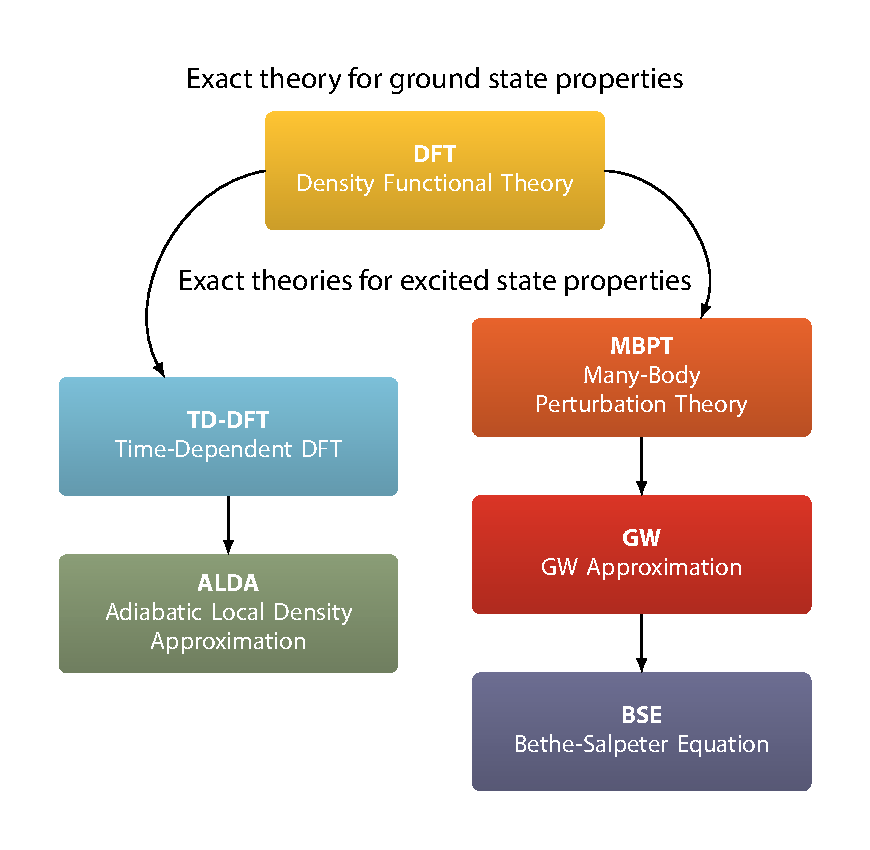
\includegraphics[height=\textheight]{diag-methods}
\end{figure}
\end{frame}

\end{document}
